\chapter{GUI编程}

\section{GUI编程}

\subsection{GUI编程}

图形用户接口GUI(Graphic User Interface)是人机交互的重要技术手段,利用GUI技术可以方便使用者使用。在不同的编程语言内部实际上也提供有一系列GUI组件。\\

如果要编写出一个图形界面,就必须非常清楚每一种组件的定义及相关的处理操作,同时还需要清除整个界面组件的布局管理。在Python中可以使用tkinter、Pyqt5组件,如果有Java的开发能力,也可以使用Jython通过Java语言类库实现图形化界面开发。在tkinter模块中提供了多种不同的窗体组件:

\begin{table}[H]
	\centering
	\setlength{\tabcolsep}{5mm}{
		\begin{tabular}{|c|l|}
			\hline
			\textbf{组件} & \textbf{描述}                        \\
			\hline
			Button        & 按钮                                 \\
			\hline
			Checkbutton   & 多选框                               \\
			\hline
			Entry         & 输入框                               \\
			\hline
			Frame         & 框架控件,在进行排版时实现子排版模型 \\
			\hline
			Label         & 标签                                 \\
			\hline
			Listbox       & 列表框                               \\
			\hline
			Menu          & 菜单                                 \\
			\hline
			Menubutton    & 菜单按钮,为菜单定义菜单项           \\
			\hline
			Radiobutton   & 单选按钮                             \\
			\hline
			Scale         & 滑动组件                             \\
			\hline
			Scrollbar     & 滚动条组件                           \\
			\hline
			Text          & 文本                                 \\
			\hline
			LabelFrame    & 容器组件,实现复杂组件布局           \\
			\hline
			tkMessageBox  & 消息组件,可以进行提示框的显示       \\
			\hline
		\end{tabular}
	}
	\caption{tkinter模块窗体组件}
\end{table}

\vspace{0.5cm}

\subsection{窗体}

任何一个图形界面都包含一个主窗体,在主窗体内可以设置不同的组件。tkinter模块中提供了Tk类,负责窗体的创建以及相关的属性定义。\\

\begin{table}[H]
	\centering
	\setlength{\tabcolsep}{4mm}{
		\begin{tabular}{|l|l|}
			\hline
			\textbf{方法}                               & \textbf{功能}            \\
			\hline
			title(self, string=None)                    & 设置窗体显示标题         \\
			\hline
			iconbitmap(self, bitmap=None, default=None) & 设置窗体logo             \\
			\hline
			geometry(self, newGeometry=None)            & 设置窗体大小             \\
			\hline
			minsize(self, width=None, height=None)      & 设置窗体最小化尺寸       \\
			\hline
			maxsize(self, width=None, height=None)      & 设置窗体最大化尺寸       \\
			\hline
			mainloop(self, n=0)                         & 界面循环及时显示窗体变化 \\
			\hline
		\end{tabular}
	}
	\caption{Tk类}
\end{table}

mainloop()的主要作用是进行窗体的显示,所有的窗体都是基于绘图的原理绘制的,所以调用此方法表示窗体进行持续的状态的显示变化。\\

\mybox{创建窗体}

\begin{lstlisting}[language=Python]
import tkinter

class MainForm:
    """
        窗体类
    """
    def __init__(self):
        self.root = tkinter.Tk()         # 创建窗体
        self.root.title("GUI编程")
        self.root.geometry("500x200")    # 初始化窗口尺寸
        self.root.maxsize(1000, 400)     # 最大尺寸
        self.root["background"] = "LightSlateGray"   # 浅青灰色
        self.root.mainloop()             # 显示窗体

def main():
    MainForm()

if __name__ == "__main__":
    main()
\end{lstlisting}

\begin{tcolorbox}
	\mybox{运行结果}
	\begin{figure}[H]
		\centering
		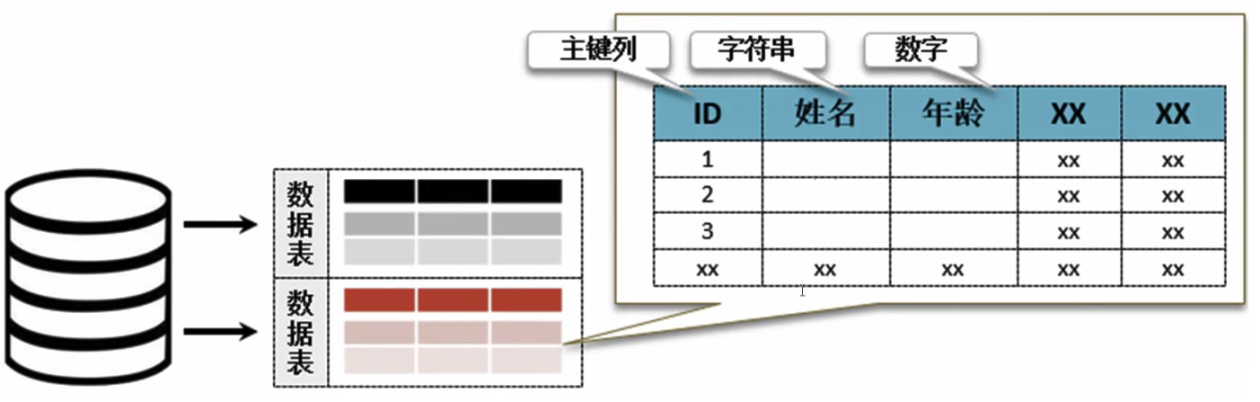
\includegraphics[]{img/C13/13-1/1.png}
	\end{figure}
\end{tcolorbox}

\vspace{0.5cm}

\subsection{基础控件}

在tkinter模块中提供了Label组件类。在一个窗体中如果要定义一些提示文字信息就可以利用标签。\\

所有的GUI组件一定要在窗体上进行各种配置,而每个组件本身有需要进行布局。如果标签没有进行布局的控制,就会按照基本的样式进行显示处理。\\

为了方便人机交互,基本都要求有一个文本输入。在tkinter模块中提供有Text组件类,这个类的最大特点就是可以进行单行文本、多行文本、图片、HTML代码的显示处理能力。\\

按钮是在图形界面之中最为常见的指令发送组件,在图形界面之中往往都是通过Text文本组件进行文字内容的输入,而后利用按钮进行相应的处理。在tkinter模块中使用Button可以实现按钮的定义。\\

\mybox{基础控件}

\begin{lstlisting}[language=Python]
import tkinter

class MainForm:
    def __init__(self):
        self.root = tkinter.Tk()
        self.root.title("GUI编程")
        self.root.geometry("500x200")

        # 标签
        self.label = tkinter.Label(
            self.root, text="用户名",
            width=10, height=5,
            font=("微软雅黑", 14)
        )

        # 文本
        self.text = tkinter.Text(
            self.root, width=20, height=1,
            font=("微软雅黑", 12)
        )
        self.text.insert(tkinter.CURRENT, "输入用户名")

        # 按钮
        self.button = tkinter.Button(self.root, text="登录")

        # 组件布局
        self.label.pack(side="left")
        self.text.pack(side="left")
        self.button.pack(side="left")

        self.root.mainloop()

def main():
    MainForm()

if __name__ == "__main__":
    main()
\end{lstlisting}

\begin{tcolorbox}
	\mybox{运行结果}
	\begin{figure}[H]
		\centering
		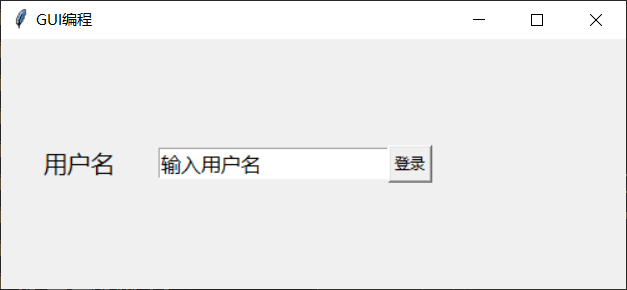
\includegraphics[]{img/C13/13-1/2.png}
	\end{figure}
\end{tcolorbox}

\newpage

\section{事件}

\subsection{事件}

图形界面中除了组件的基本展示之外,最为重要的就是要定义与组件有关的事件处理操作。在tkinter中可以方便地为每一个组件进行事件绑定,并且设置事件的相关处理函数,这样每当触发相应的事件之后就可以通过特定地函数实现事件处理。

\begin{figure}[H]
	\centering
	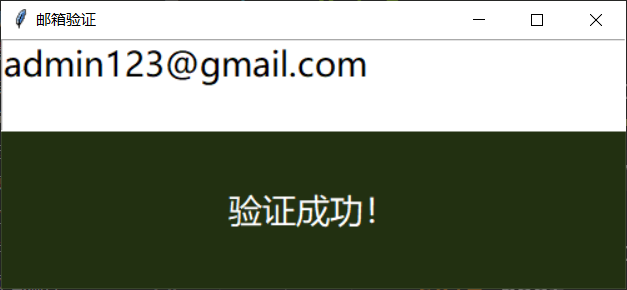
\includegraphics[]{img/C13/13-2/1.png}
\end{figure}

当事件触发后会产生一个事件对象,利用这个事件对象可以在处理函数中获得相应的数据信息,例如哪一个组件触发的操作、操作的坐标等。\\

通过使用bind()可以进行事件的绑定,而在绑定的时候一定要有每一个方法对应的事件的类型,事件的类型是由tkinter规定好的。

\begin{table}[H]
	\centering
	\setlength{\tabcolsep}{5mm}{
		\begin{tabular}{|c|l|}
			\hline
			\textbf{事件} & \textbf{功能}                  \\
			\hline
			Button        & 当用户点击鼠标按键时触发       \\
			\hline
			ButtonRelease & 鼠标按键松开时触发             \\
			\hline
			Enter         & 当鼠标指针进入组件时触发       \\
			\hline
			FocusIn       & 当组件获得焦点时触发           \\
			\hline
			FocusOut      & 当组件失去焦点时触发           \\
			\hline
			KeyPress      & 当键盘按下时触发               \\
			\hline
			KeyRelease    & 当按键松开时触发               \\
			\hline
			Leave         & 当鼠标指针离开组件时触发       \\
			\hline
			Motion        & 当鼠标在组件内部移动时触发     \\
			\hline
			Visibility    & 当应用组件可见时触发           \\
			\hline
			MouseWheel    & 当鼠标在组件内部滚轮滚动时触发 \\
			\hline
		\end{tabular}
	}
	\caption{事件}
\end{table}

\vspace{0.5cm}

\mybox{验证邮箱合法性}

\begin{lstlisting}[language=Python]
import  tkinter
import  re

#  合法邮箱正则语法
EMAIL  =  "[a-zA-Z0-9]\\w+@\\w+\\.(cn|com|com.cn|gov|net)"

class  MainForm:
    def  __init__(self):
        self.root  =  tkinter.Tk()
        self.root.title("邮箱验证")
        self.root.geometry("500x200")

        self.text  =  tkinter.Text(
            self.root,  width=500,  height=2,
            font=("微软雅黑",  20)
        )
        #  提示信息
        self.text.insert("current",  "输入邮箱")
        #  鼠标单击后删除文本组件中的全部内容
        self.text.bind("<Button-1>",  
            lambda  event:  self.text.delete("0.0",  "end"))
        #  绑定键盘事件
        self.text.bind("<KeyPress>",  
            lambda  event:  self.keyboard_event_handler(event))
        self.text.bind("<KeyRelease>",  
            lambda  event:  self.keyboard_event_handler(event))
        self.text.pack()

        self.content  =  tkinter.StringVar()      #  修改标签文字
        
        self.label  =  tkinter.Label(
            self.root,  width=200,  height=200,
            textvariable=self.content,
            bg="#223011",  fg="#ffffff",
            font=("微软雅黑",  20)
        )
        self.label.pack()

        self.root.mainloop()
    
    def  keyboard_event_handler(self,  event):
        """
            键盘处理时间
            Args:
                event:  事件
        """
        #  获取文本框数据
        email  =  self.text.get("0.0",  "end")
        if  re.match(EMAIL,  email):
            self.content.set("验证成功!")
        else:
            self.content.set("格式错误!")

def  main():
    MainForm()
    
if  __name__  ==  "__main__":
    main()
\end{lstlisting}

\begin{tcolorbox}
	\mybox{运行结果}
	\begin{figure}[H]
		\centering
		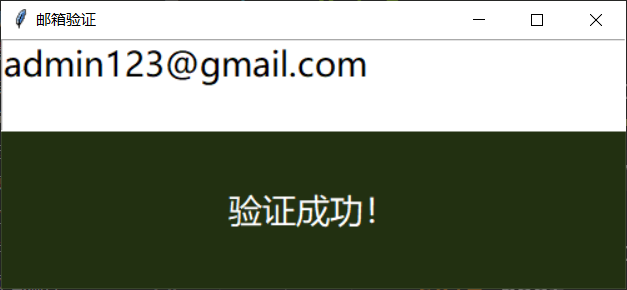
\includegraphics[]{img/C13/13-2/2.png}
	\end{figure}
\end{tcolorbox}

\newpage

\section{布局}

\subsection{pack布局}

pack布局是GUI布局之中最为常见的一种形式,这种布局属于顺序式排列布局。如果没有引入布局管理器的概念,实际上组件是不会显示的。如果没有对布局管理器进行合理的配置,显示的效果就会非常混乱。

\begin{table}[H]
	\centering
	\setlength{\tabcolsep}{3mm}{
		\begin{tabular}{|c|l|l|}
			\hline
			\textbf{参数} & \textbf{取值范围}                  & \textbf{功能}          \\
			\hline
			fill          & none、x、y、both                   & 是否水平或垂直方向填充 \\
			\hline
			expand        & yes(1)、no(0)                  & 是否可以展开           \\
			\hline
			side          & left、right、top、bottom           & 摆放位置               \\
			\hline
			anchor        & n、s、w、e、nw、ne、sw、se、center & 设置在窗体中八个方位   \\
			\hline
		\end{tabular}
	}
	\caption{pack布局}
\end{table}

\vspace{0.5cm}

\mybox{pack布局}

\begin{lstlisting}[language=Python]
import tkinter

class MainForm:
    def __init__(self):
        self.root = tkinter.Tk()
        self.root.title("GUI编程")
        self.root.geometry("500x200")

        label = tkinter.Label(
            self.root, text="用户名",
            width=10, height=2,
            font=("微软雅黑", 14)
        )
        text = tkinter.Text(
            self.root, width=20, height=2,
            font=("微软雅黑", 14)
        )
        text.insert("current", "输入用户名")

        label.pack(side="top")
        text.pack(side="bottom")
        self.root.mainloop()

def main():
    MainForm()

if __name__ == "__main__":
    main()
\end{lstlisting}

\begin{tcolorbox}
	\mybox{运行结果}
	\begin{figure}[H]
		\centering
		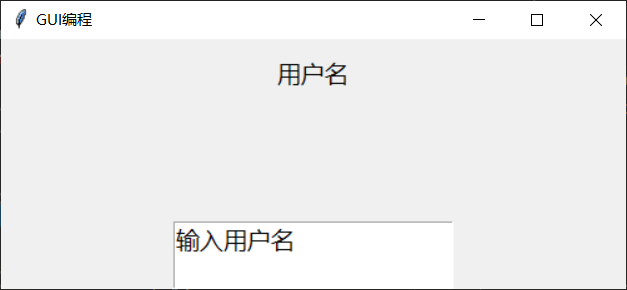
\includegraphics[]{img/C13/13-3/1.png}
	\end{figure}
\end{tcolorbox}

\vspace{0.5cm}

\subsection{grid布局}

grid布局利用表结构的形式来实现布局的管理,在一张数据表里面一定会有行和列,在使用grid布局的时候就可以通过行和列实现组件的摆放。\\

计算器实际上就属于一种grid布局的形式:

\begin{figure}[H]
	\centering
	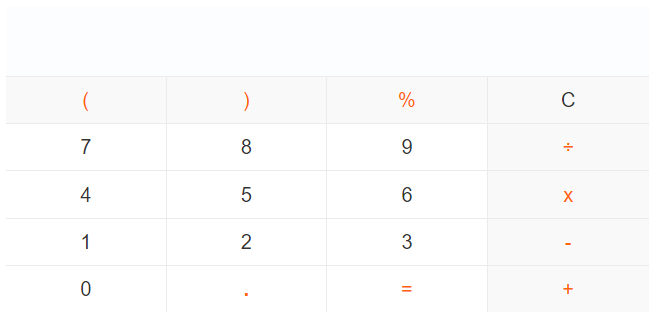
\includegraphics[]{img/C13/13-3/2.png}
	\caption{计算器}
\end{figure}

\vspace{0.5cm}

\mybox{grid布局}

\begin{lstlisting}[language=Python]
import tkinter

class MainForm:
    def __init__(self):
        self.root = tkinter.Tk()
        self.root.title("GUI编程")
        self.root.geometry("500x200")
        label1 = tkinter.Label(self.root, text="标签1")
        label2 = tkinter.Label(self.root, text="标签2")
        label1.grid(row=0, column=0)
        label2.grid(row=1, column=1)
        self.root.mainloop()

def main():
    MainForm()

if __name__ == "__main__":
    main()
\end{lstlisting}

\begin{tcolorbox}
	\mybox{运行结果}
	\begin{figure}[H]
		\centering
		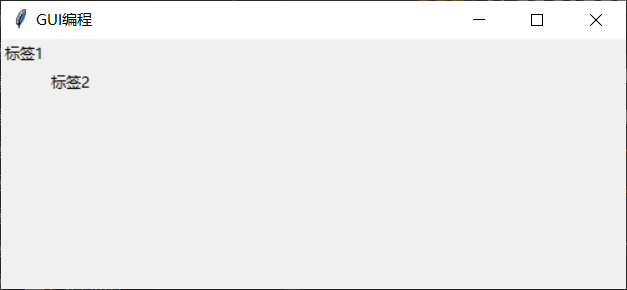
\includegraphics[]{img/C13/13-3/3.png}
	\end{figure}
\end{tcolorbox}

\vspace{0.5cm}

\subsection{place布局}

place布局是布局管理器之中最灵活的一种布局形式,它采用的是坐标点位置的布局操作。\\

\mybox{place布局}

\begin{lstlisting}[language=Python]
import tkinter

class MainForm:
    def __init__(self):
        self.root = tkinter.Tk()
        self.root.title("GUI编程")
        self.root.geometry("500x200")
        label = tkinter.Label(self.root, text="标签")
        label.place(x=100, y=50)
        self.root.mainloop()

def main():
    MainForm()

if __name__ == "__main__":
    main()
\end{lstlisting}

\begin{tcolorbox}
	\mybox{运行结果}
	\begin{figure}[H]
		\centering
		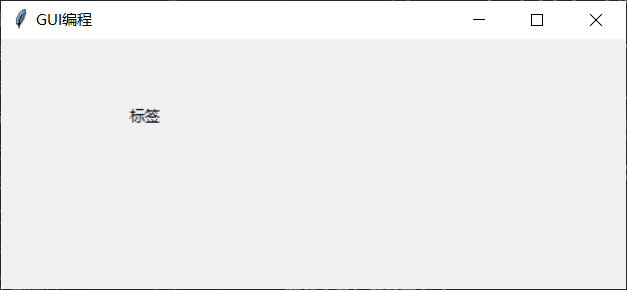
\includegraphics[]{img/C13/13-3/4.png}
	\end{figure}
\end{tcolorbox}

\vspace{0.5cm}

\subsection{Frame}

Frame是布局管理最为重要的一项布局技术,但是Frame本身并不是布局,而是一种内嵌的布局管理器。在一个窗体中针对不同的功能组件定义一个单独的区域,每一个区域相当于就是一个Frame,这些区域的内部都可以使用不同的布局管理器。

\begin{figure}[H]
	\centering
	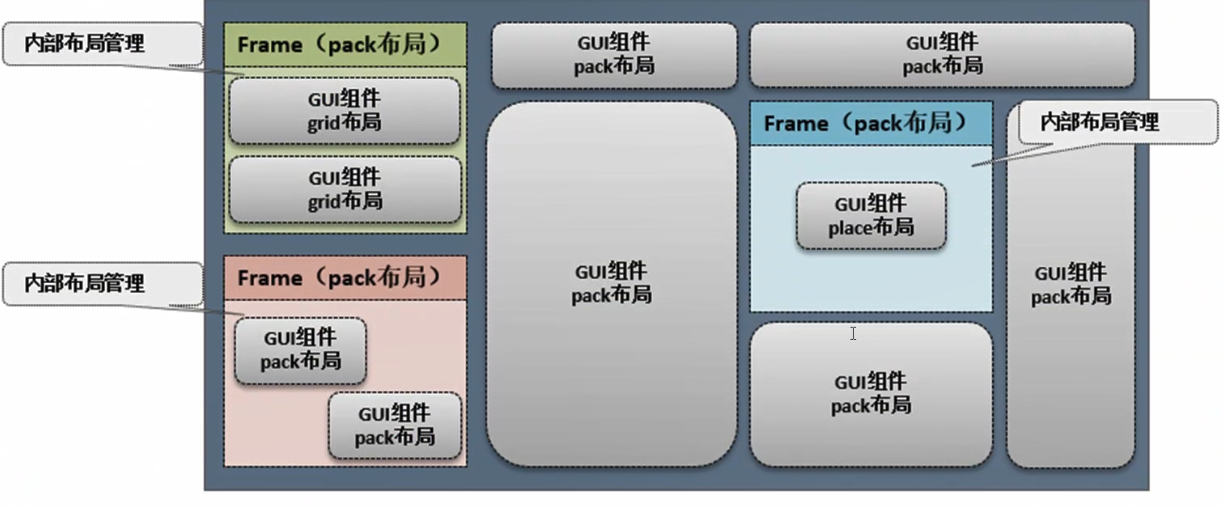
\includegraphics[scale=0.6]{img/C13/13-3/5.png}
\end{figure}

最具有代表性的Frame程序就是Windows中的计算器:

\begin{figure}[H]
	\centering
	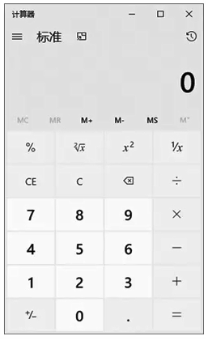
\includegraphics[]{img/C13/13-3/6.png}
	\caption{计算器}
\end{figure}

\vspace{0.5cm}

\mybox{计算器}

\begin{lstlisting}[language=Python]
import tkinter
import re

class MainForm:
    def __init__(self):
        self.root = tkinter.Tk()
        self.root.title("计算器")
        self.root.geometry("231x280")
        self.input_frame()      # 输入区
        self.button_frame()     # 按钮区
        self.root.mainloop()
    
    def input_frame(self):
        """
            输入区
        """
        # 创建内部容器
        self.in_frame = tkinter.Frame(self.root, width=20)
        self.content = tkinter.StringVar()
        # 单行输入
        self.entry = tkinter.Entry(
            self.in_frame, width=14,
            font=("微软雅黑", 20),
            textvariable=self.content
        )
        self.entry.pack(fill="x", expand=1)
        # 清除标记,每一次计算完成后清除
        self.clean = False
        self.in_frame.pack(side="top")
    
    def button_frame(self):
        """
            按钮区
        """
        self.btn_frame = tkinter.Frame(self.root, width=50)
        self.button_list = [[], [], [], []]     # 4行4列
        button = "123+456-789*0.=/"
        
        for row in range(4):
            for col in range(4):
                self.button_list[row].append(
                    tkinter.Button(
                        self.btn_frame,
                        text=button[4*row+col],
                        fg="black", width=3,
                        font=("微软雅黑", 20),
                    )
                )
        
        self.row = 0
        for group in self.button_list:
            self.column = 0
            for button in group:
                # 绑定事件
                button.bind(
                    "<Button-1>", 
                    lambda event: self.button_handler(event)
                )
                button.grid(row=self.row, column=self.column)
                self.column += 1
            self.row += 1
        self.btn_frame.pack(side="bottom")

    def button_handler(self, event):
        """
            按键事件处理
            Args:
                event: 单击事件
        """
        op = event.widget["text"]   # 获取按钮内容

        if self.clean:      # 新一次计算
            self.content.set("")    # 清除数据
            self.clean = False
        
        if op != "=":
            self.entry.insert("end", op)
        elif op == "=":
            result = 0
            expression = self.entry.get()
            pattern = r"\+|\-|\*|\/"

            nums = re.split(pattern, expression)
            op = re.findall(pattern, expression)[0]

            if op == "+":
                result = float(nums[0]) + float(nums[1])
            elif op == "-":
                result = float(nums[0]) - float(nums[1])
            elif op == "*":
                result = float(nums[0]) * float(nums[1])
            elif op == "/":
                result = float(nums[0]) / float(nums[1])
                
            self.entry.insert("end", "=%s" % result)
            self.clean = True

def main():
    MainForm()

if __name__ == "__main__":
    main()
\end{lstlisting}

\begin{tcolorbox}
	\mybox{运行结果}
	\begin{figure}[H]
		\centering
		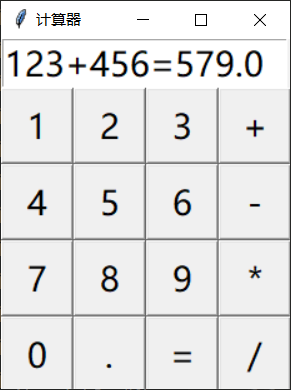
\includegraphics[]{img/C13/13-3/7.png}
	\end{figure}
\end{tcolorbox}

\newpage

\section{组件}

\subsection{列表(Listbox)}

Listbox是进行列表显示的组件,可以向列表中添加多个列表项,这些列表项会依次排列。列表项可以进行动态的控制(添加、删除),还可以设置列表项是单选还是多选。

\begin{table}[H]
	\centering
	\setlength{\tabcolsep}{5mm}{
		\begin{tabular}{|l|c|l|}
			\hline
			\textbf{名称}  & \textbf{类型} & \textbf{功能}              \\
			\hline
			BROWSE         & 常量          & 每次只能选择一项,可以拖动 \\
			\hline
			SINGLE         & 常量          & 每次只能选择一项,不能拖动 \\
			\hline
			MULTIPLE       & 常量          & 每次可以选择多项           \\
			\hline
			insert()       & 方法          & 追加列表项                 \\
			\hline
			curselection() & 方法          & 获取选中列表项索引         \\
			\hline
			delete()       & 方法          & 删除指定索引的列表项       \\
			\hline
		\end{tabular}
	}
	\caption{Listbox}
\end{table}

\vspace{0.5cm}

\mybox{Listbox}

\begin{lstlisting}[language=Python]
import tkinter

class MainForm:
    def __init__(self):
        self.root = tkinter.Tk()
        self.root.geometry("500x200")
        self.src_list()     # 待选区
        self.dst_list()     # 已选区
        self.set_button()   # 按钮区
        self.root.mainloop()
    
    def src_list(self):
        """
            待选区列表
        """
        self.src_label = tkinter.Label(
            self.root,
            text="选择擅长的编程语言",
            bg="#223011", fg="#fff",
            font=("微软雅黑", 9)
        )
        self.src_label.grid(row=0, column=0)
        self.languages = [
            "Python", "Java", "JavaScript",
            "C", "C++", "PHP", "Go", 
        ]
        self.language_listbox = tkinter.Listbox(
            self.root, selectmode="multiple"
        )
        for language in self.languages:
            self.language_listbox.insert("end", language)
        # 双击选中
        self.language_listbox.bind(
            "<Double-Button-1>", self.add_handler
        )
        self.language_listbox.grid(row=1, column=0)
    
    def dst_list(self):
        """
            已选区列表
        """
        self.dst_label = tkinter.Label(
            self.root, text="擅长的编程语言",
            bg="#223011", fg="#fff",
            font=("微软雅黑", 9)
        )
        self.dst_label.grid(row=0, column=3)
        self.selected_listbox = tkinter.Listbox(
            self.root, selectmode="multiple"
        )
        self.selected_listbox.grid(row=1, column=3)
    
    def set_button(self):
        """
            设置按钮
        """
        self.add_btn = tkinter.Button(
            self.root, text="添加 >>",
            fg="#000", font=("微软雅黑", 9)
        )
        self.add_btn.bind("<Button-1>", self.add_handler)
        self.add_btn.grid(row=1, column=1)
    
    def add_handler(self, event):
        """
            添加按钮事件处理
        """
        # 获取全部被选中的数据索引
        for index in self.language_listbox.curselection():
            self.selected_listbox.insert(
                "end", self.language_listbox.get(index)
            )
        # 索引在每一次删除之后都会动态改变
        while True:
            # 有被选中的项
            if self.language_listbox.curselection():
                # 删除当前项
                self.language_listbox.delete(
                    self.language_listbox.curselection()[0]
                )
            else:
                break

def main():
    MainForm()

if __name__ == "__main__":
    main()
\end{lstlisting}

\begin{tcolorbox}
	\mybox{运行结果}
	\begin{figure}[H]
		\centering
		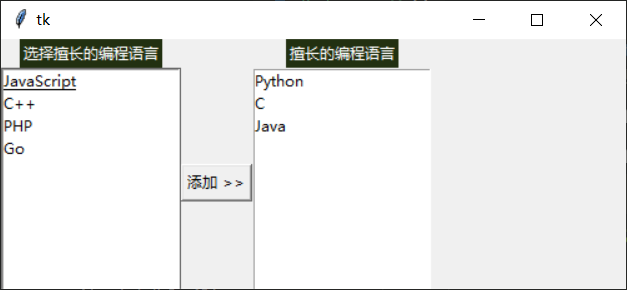
\includegraphics[]{img/C13/13-4/1.png}
	\end{figure}
\end{tcolorbox}

\vspace{0.5cm}

\subsection{单选钮(Radiobutton)}

Radiobutton实现了单选钮的操作,给定若干的选项,但是只允许选择一项,这些选项属于互斥的状态。\\

\mybox{Radiobutton}

\begin{lstlisting}[language=Python]
import tkinter

class MainForm:
    def __init__(self):
        self.root = tkinter.Tk()
        self.root.geometry("500x200")

        # 单选按钮需要设置显示内容和对应数据值
        self.sex = [("男", 0), ("女", 1)]

        self.label = tkinter.Label(
            self.root, text="选择性别:",
            font=("微软雅黑", 14)
        )
        self.label.grid(row=0, column=0)

        pos = 1
        for title, index in self.sex:
            radio = tkinter.Radiobutton(
                self.root, font=("微软雅黑", 14),
                text=title, value=index,
            )
            radio.grid(row=0, column=pos)
            pos += 1

        self.root.mainloop()

def main():
    MainForm()

if __name__ == "__main__":
    main()
\end{lstlisting}

\begin{tcolorbox}
	\mybox{运行结果}
	\begin{figure}[H]
		\centering
		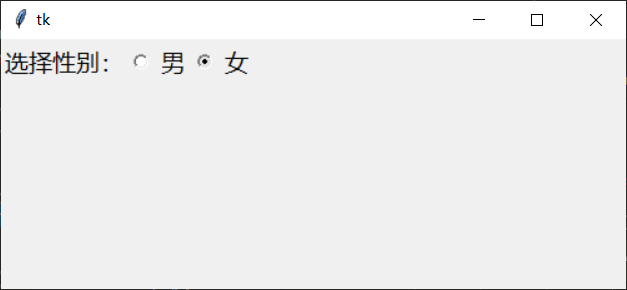
\includegraphics[]{img/C13/13-4/2.png}
	\end{figure}
\end{tcolorbox}

\vspace{0.5cm}

\subsection{复选框(Checkbutton)}

复选框每次可以同时选择多个数据项。\\

\mybox{Checkbutton}

\begin{lstlisting}[language=Python]
import tkinter

class MainForm:
    def __init__(self):
        self.root = tkinter.Tk()
        self.root.geometry("500x200")

        self.label = tkinter.Label(
            self.root, text="选择擅长的编程语言",
            font=("微软雅黑", 12)
        )
        self.label.pack(anchor="w")

        self.language = [
            ("Java", tkinter.IntVar()),
            ("Python", tkinter.IntVar()),
            ("C", tkinter.IntVar()),
            ("C++", tkinter.IntVar()),
            ("JavaScript", tkinter.IntVar())
        ]
        for title, status in self.language:
            check = tkinter.Checkbutton(
                self.root,
                text=title, variable=status,
                onvalue=1, offvalue=0,
                command=self.select_handler
            )
            check.pack(anchor="w")
        
        self.content = tkinter.StringVar()
        self.show_label = tkinter.Label(
            self.root, font=("微软雅黑", 12),
            textvariable=self.content,
        )
        self.show_label.pack(anchor="w")

        self.root.mainloop()
    
    def select_handler(self):
        result = "擅长的技术:"
        for title, status in self.language:
            if status.get() == 1:   # 选中为1
                result += title + " "
        self.content.set(result)

def main():
    MainForm()

if __name__ == "__main__":
    main()
\end{lstlisting}

\begin{tcolorbox}
	\mybox{运行结果}
	\begin{figure}[H]
		\centering
		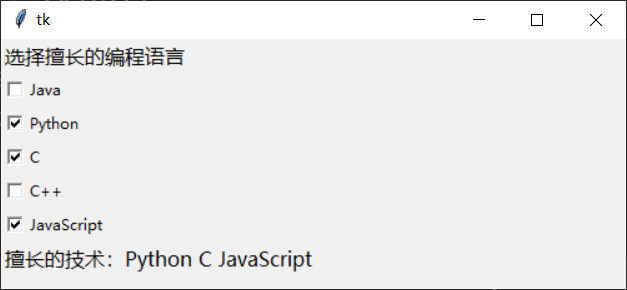
\includegraphics[]{img/C13/13-4/3.png}
	\end{figure}
\end{tcolorbox}

\vspace{0.5cm}

\subsection{滑块(Scale)}

tkinter.Scale是一个滑块组件,像操作系统中经常使用滑块拖动的形式修改音量大小。Scale定义了一个区间范围,区间的数值是通过Scale进行控制的。\\

\mybox{Scale}

\begin{lstlisting}[language=Python]
import tkinter

class MainForm:
    def __init__(self):
        self.root = tkinter.Tk()
        self.root.geometry("500x200")

        self.label = tkinter.Label(
            self.root, text="测试文本", 
            font=("微软雅黑", 1), fg="#f00"
        )
        self.label.pack(anchor="w")

        self.scale = tkinter.Scale(
            self.root, label="拖动调整文字大小",
            from_=0, to=20,
            orient=tkinter.HORIZONTAL,
            length=300, tickinterval=2,
            showvalue=True, resolution=True
        )
        self.scale.bind("<B1-Motion>", self.font_handler)
        self.scale.pack(anchor="s")

        self.root.mainloop()
    
    def font_handler(self, event):
        self.label.config(font=("微软雅黑", self.scale.get()))

def main():
    MainForm()

if __name__ == "__main__":
    main()
\end{lstlisting}

\begin{tcolorbox}
	\mybox{运行结果}
	\begin{figure}[H]
		\centering
		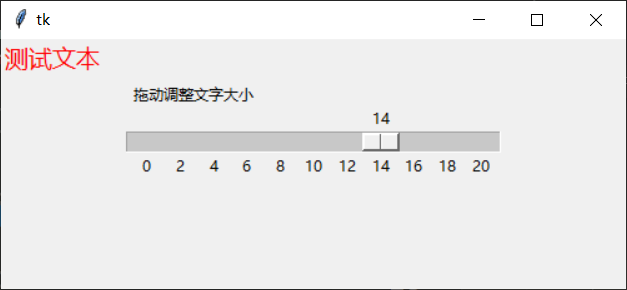
\includegraphics[]{img/C13/13-4/4.png}
	\end{figure}
\end{tcolorbox}

\vspace{0.5cm}

\subsection{滚动条(Scrollbar)}

Scrollbar是一个滚动条组件,它并不是一种固定的组件,而是一种辅助功能组件。例如列表项内容过多,通过滚动条的形式就可以方便地进行控制。\\

\mybox{Scrollbar}

\begin{lstlisting}[language=Python]
import tkinter

class MainForm:
    def __init__(self):
        self.root = tkinter.Tk()
        self.root.geometry("500x200")

        self.label = tkinter.Label(
            self.root, text="内容",
            font=("微软雅黑", 12)
        )
        self.label.pack(anchor="nw")

        self.frame = tkinter.Frame(self.root)   # 内部容器
        self.listbox = tkinter.Listbox(
            self.frame,
            height=5, width=80
        )
        for i in range(100):
            self.listbox.insert(tkinter.END, "item %d" % i)
        
        self.scrollbar = tkinter.Scrollbar(self.frame)
        self.scrollbar.config(command=self.listbox.yview)
        self.scrollbar.pack(side="right", fill="y")
        self.listbox.pack()
        self.frame.pack(anchor="w")

        self.root.mainloop()

def main():
    MainForm()

if __name__ == "__main__":
    main()
\end{lstlisting}

\begin{tcolorbox}
	\mybox{运行结果}
	\begin{figure}[H]
		\centering
		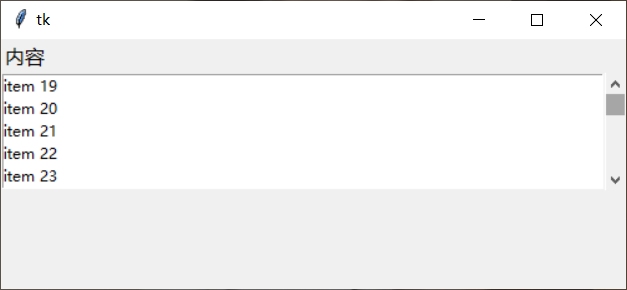
\includegraphics[]{img/C13/13-4/5.png}
	\end{figure}
\end{tcolorbox}

\vspace{0.5cm}

\subsection{菜单(Menu)}

菜单可以充分发挥出界面开发的优势,同时也可以极大地改善界面布局。

\begin{table}[H]
	\centering
	\setlength{\tabcolsep}{5mm}{
		\begin{tabular}{|l|l|}
			\hline
			\textbf{方法}    & \textbf{描述}  \\
			\hline
			add\_command()   & 追加菜单项     \\
			\hline
			add\_separator() & 菜单分割线     \\
			\hline
			add\_cascade()   & 追加子菜单     \\
			\hline
			post()           & 弹出式菜单显示 \\
			\hline
			insert()         & 追加菜单项     \\
			\hline
		\end{tabular}
	}
	\caption{Menu}
\end{table}

\vspace{0.5cm}

\mybox{Menu}

\begin{lstlisting}[language=Python]
import tkinter

class MainForm:
    def __init__(self):
        self.root = tkinter.Tk()
        self.root.geometry("500x200")
        self.create_menu()
        self.root.mainloop()
    
    def create_menu(self):
        self.menu = tkinter.Menu(self.root)

        self.file_menu = tkinter.Menu(self.menu, tearoff=False)
        self.file_menu.add_command(
            label="打开", 
            command=self.menu_handler
        )
        self.file_menu.add_command(
            label="保存", 
            command=self.menu_handler
        )
        self.file_menu.add_separator()
        self.file_menu.add_command(
            label="关闭", 
            command=self.root.quit
        )
        self.menu.add_cascade(
            label="文件", 
            menu=self.file_menu
        )

        self.edit_menu = tkinter.Menu(self.menu, tearoff=False)
        self.edit_menu.add_command(
            label="剪切", 
            command=self.menu_handler
         )
        self.edit_menu.add_command(
            label="复制", 
            command=self.menu_handler
         )
        self.edit_menu.add_command(
            label="粘贴", 
            command=self.menu_handler
        )
        self.edit_menu.add_separator()
        self.edit_menu.add_command(
            label="设置", 
            command=self.root.quit
        )
        self.menu.add_cascade(
            label="编辑", 
            menu=self.edit_menu
        )

        self.root.config(menu=self.menu)

        self.pop_menu = tkinter.Menu(self.root, tearoff=False)
        self.pop_menu.add_command(
            label="帮助", 
            command=self.popup_handler
        )
        self.root.bind("<Button-3>", self.popup_handler)
    
    def menu_handler(self):
        pass

    def popup_handler(self, event):
        self.pop_menu.post(event.x_root, event.y_root)

def main():
    MainForm()

if __name__ == "__main__":
    main()
\end{lstlisting}

\begin{tcolorbox}
	\mybox{运行结果}
	\begin{figure}[H]
		\centering
		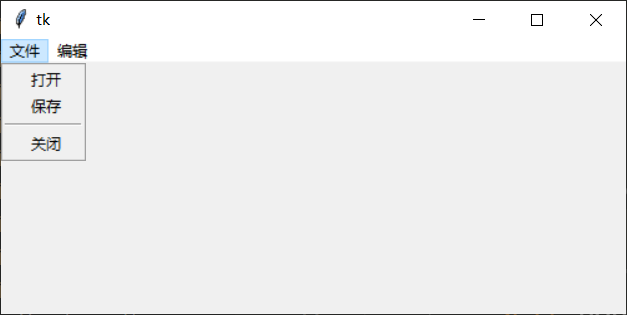
\includegraphics[]{img/C13/13-4/6.png}
	\end{figure}
\end{tcolorbox}

\newpage

\section{graphics}

\subsection{graphics}

graphics是一个第三方组件,这个组件提供有专门的绘图支持。\\

\mybox{四则运算}

\begin{lstlisting}[language=Python]
import graphics

def main():
    win = graphics.GraphWin("四则运算", 700, 230)

    # 数字1输入框
    graphics.Text(graphics.Point(80, 50), "数字1").draw(win)
    input_num1 = graphics.Entry(graphics.Point(160, 50), 8)
    input_num1.setFill("white")     # 输入框底色
    input_num1.setText("0.0")
    input_num1.draw(win)

    # 数字2输入框
    graphics.Text(graphics.Point(280, 50), "数字2").draw(win)
    input_num2 = graphics.Entry(graphics.Point(360, 50), 8)
    input_num2.setFill("white")     # 输入框底色
    input_num2.setText("0.0")
    input_num2.draw(win)

    # 提示信息
    graphics.Text(graphics.Point(80, 100), "【四则运算】").draw(win)

    # 加法
    graphics.Text(graphics.Point(120, 150), "加法").draw(win)
    output_add = graphics.Entry(graphics.Point(250, 150), 15)
    output_add.setFill("white")
    output_add.draw(win)

    # 减法
    graphics.Text(graphics.Point(400, 150), "减法").draw(win)
    output_sub = graphics.Entry(graphics.Point(530, 150), 15)
    output_sub.setFill("white")
    output_sub.draw(win)

    # 乘法
    graphics.Text(graphics.Point(120, 200), "乘法").draw(win)
    output_mul = graphics.Entry(graphics.Point(250, 200), 15)
    output_mul.setFill("white")
    output_mul.draw(win)

    # 除法
    graphics.Text(graphics.Point(400, 200), "除法").draw(win)
    output_div = graphics.Entry(graphics.Point(530, 200), 15)
    output_div.setFill("white")
    output_div.draw(win)

    # 鼠标单击开始计算
    win.getMouse()

    # 计算并显示结果
    output_add.setText(
        eval(input_num1.getText()) + eval(input_num2.getText())
    )
    output_sub.setText(
        eval(input_num1.getText()) - eval(input_num2.getText())
    )
    output_mul.setText(
        eval(input_num1.getText()) * eval(input_num2.getText())
    )
    output_div.setText(
        eval(input_num1.getText()) / eval(input_num2.getText())
    )

    win.mainloop()

if __name__ == "__main__":
    main()
\end{lstlisting}

\begin{tcolorbox}
	\mybox{运行结果}
	\begin{figure}[H]
		\centering
		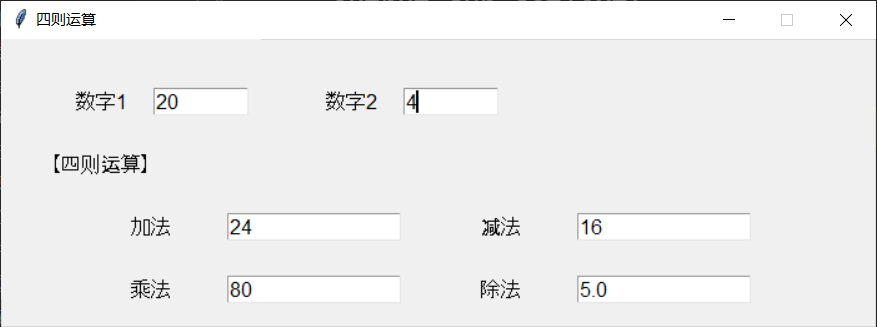
\includegraphics[scale=0.7]{img/C13/13-5/1.png}
	\end{figure}
\end{tcolorbox}

\newpage

\section{turtle}

\subsection{turtle}

海龟绘图turtle模块是最有特色的一个第三方模块,这个模块可以让整个程序变得非常生动。\\

\mybox{绘制五角星}

\begin{lstlisting}[language=Python]
import turtle

def main():
    turtle.shape(name="turtle")     # 使用海龟作为画笔
    turtle.Screen().title("五角星")
    turtle.Screen().bgcolor("red")  # 背景色
    turtle.pensize(3)               # 画笔大小
    turtle.pencolor("yellow")       # 画笔颜色
    turtle.fillcolor("yellow")      # 填充色

    turtle.begin_fill()             # 开始填充
    for _ in range(5):              # 绘制5条线
        turtle.forward(320)         # 向前移动
        turtle.right(144)           # 向右旋转144°
    turtle.end_fill()               # 结束填充

    turtle.penup()                  # 抬起画笔
    turtle.goto(-200, -120)         # 移动位置
    turtle.color("white")
    turtle.write("Turtle", font=("微软雅黑", 20))
    turtle.mainloop()

if __name__ == "__main__":
    main()
\end{lstlisting}

\begin{tcolorbox}
	\mybox{运行结果}
	\begin{figure}[H]
		\centering
		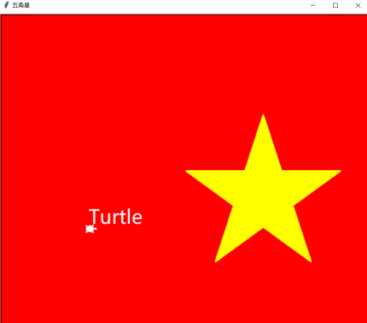
\includegraphics[]{img/C13/13-6/1.png}
	\end{figure}
\end{tcolorbox}

\vspace{0.5cm}

\mybox{迷宫}

\begin{lstlisting}[title=maze.txt]
0 0 0 0 0 0 0 0 0 0 0 0 0 0 0 0 0 0 0 0 0 0 0 0 0 0 0 0 0 0 0 0 0
0 1 1 1 0 1 0 1 1 1 1 1 0 1 1 1 1 1 0 1 1 1 0 1 1 1 1 1 1 1 1 1 0
0 1 0 1 0 1 0 1 0 0 0 0 0 1 0 0 0 0 0 1 0 0 0 1 0 0 0 0 0 1 0 0 0
0 0 1 1 1 1 1 1 0 1 1 1 1 1 1 1 1 1 0 1 0 1 1 1 1 1 1 1 0 1 1 1 0
0 0 0 1 0 0 0 0 0 0 0 1 0 0 0 1 0 0 0 1 0 1 0 1 0 1 0 1 0 0 0 1 0
0 0 1 S 1 1 1 1 1 1 1 1 0 1 0 1 1 1 1 1 1 1 0 1 0 1 0 1 1 1 0 1 0
0 0 0 1 0 1 0 0 0 0 0 0 0 1 0 1 0 0 0 1 0 1 0 1 0 1 0 1 0 1 0 1 0
0 0 1 1 0 1 1 1 0 1 1 1 1 1 0 1 1 1 0 1 0 1 0 1 0 1 0 1 1 1 0 1 0
0 0 0 1 0 1 0 0 0 1 0 1 0 1 0 0 0 0 0 1 0 D 0 1 0 1 0 0 0 1 0 0 0
0 0 1 1 0 1 1 1 1 1 0 1 0 1 1 1 0 1 0 1 0 1 0 1 0 1 1 1 0 1 0 1 0
0 0 0 1 0 1 0 1 0 1 0 0 0 0 0 0 0 1 0 0 0 1 0 1 0 1 0 0 0 1 0 1 0
0 0 1 1 0 1 0 1 0 1 1 1 1 1 1 1 1 1 1 1 0 1 0 1 0 1 1 1 0 1 1 1 0
0 0 0 1 0 0 0 0 0 1 0 0 0 0 0 1 0 1 0 0 0 0 0 0 0 0 0 0 0 1 0 1 0
0 0 1 1 0 1 1 1 1 1 1 1 1 1 0 1 0 1 1 1 1 1 1 1 1 1 1 1 0 1 0 1 0
0 0 0 0 0 1 0 1 0 1 0 1 0 1 0 1 0 1 0 1 0 0 0 1 0 1 0 0 0 1 0 0 0
0 0 1 1 1 1 0 1 0 1 0 1 0 1 0 1 0 1 0 1 0 1 1 1 0 1 1 1 0 1 0 1 0
0 0 0 0 0 1 0 0 0 0 0 0 0 0 0 0 0 1 0 1 0 0 0 1 0 0 0 1 0 1 0 1 0
0 0 1 1 1 1 1 1 1 1 1 1 1 1 0 1 0 1 0 1 0 1 1 1 1 1 0 1 0 1 1 1 0
0 0 0 1 0 0 0 0 0 1 0 0 0 0 0 1 0 0 0 1 0 1 0 1 0 0 0 1 0 0 0 1 0
0 0 1 1 0 1 1 1 1 1 1 1 1 1 1 1 1 1 0 1 0 1 0 1 1 1 0 1 0 1 1 1 0
0 0 0 0 0 0 0 0 0 0 0 0 0 0 0 0 0 0 0 0 0 0 0 0 0 0 0 0 0 0 0 0 0
\end{lstlisting}

\begin{lstlisting}[language=Python, title=maze.txt]
import turtle
import random

MAZE_FILE = "maze.txt"

class Maze:
    CELL_SIZE = 20      # 单元格尺寸

    def __init__(self, path):
        """
            从文件中获取迷宫数据
            s Args:
                path (str): 迷宫数据路径
        """
        with open(path) as file:
            lines = file.readlines()
        self.maze_data = [line.strip().split(' ') for line in lines]
        self.row = len(self.maze_data)
        self.col = len(self.maze_data[0])
        self.src_x = self.src_y = 0     # 起点坐标
        self.src_row = self.src_col = 0 # 起点行列
    
    def goto(self, x, y, pen):
        pen.up()
        pen.goto(x, y)
        pen.down()

    def draw_maze(self):
        """
            绘制迷宫
        """
        self.screen = turtle.Screen()
        self.screen.title("迷宫")
        self.screen.colormode(255)       # 颜色模式
        self.screen.tracer(0)            # 关闭动画
        self.screen.setup(
            self.col * self.CELL_SIZE, 
            self.row * self.CELL_SIZE
        )

        self.pen = turtle.Turtle()  # 画笔
        self.pen.pensize(self.CELL_SIZE * 0.2)  # 画笔大小
        self.pen.hideturtle()       # 隐藏海龟

        for i in range(self.row):
            for j in range(self.col):
                # 墙
                if self.maze_data[i][j] == '0':
                    self.draw_cell(j, i)
                # 起点(Src)
                elif self.maze_data[i][j] == 'S':
                    # 设置起点坐标
                    self.src_x 
                        = (j - self.col * 0.5 + 0.5) * self.CELL_SIZE
                    self.src_y 
                        = (self.row * 0.5 - i - 0.5) * self.CELL_SIZE
                    # 设置起点所在行列
                    self.src_row = i
                    self.src_col = j
                    self.draw_point(j, i, "purple")
                # 终点(Destination)
                elif self.maze_data[i][j] == 'D':
                    self.draw_point(j, i, "red")
        
    def draw_cell(self, col, row):
        """
            绘制单元格
            Args:
                col (int): 列
                row (int): 行
        """
        x = (col - self.col * 0.5) * self.CELL_SIZE
        y = (self.row * 0.5 - row) * self.CELL_SIZE
        self.goto(x, y, self.pen)

        n = random.randint(110, 150)
        self.pen.color((n, n, n), (n, n, n))
        self.pen.begin_fill()
        for _ in range(4):
            self.pen.forward(self.CELL_SIZE)
            self.pen.right(90)
        self.pen.end_fill()
    
    def draw_point(self, col, row, color):
        """
            绘制起点/终点
            Args:
                col (int): 列
                row (int): 行
                color (str): 点的颜色
        """
        x = (col - self.col * 0.5 + 0.5) * self.CELL_SIZE
        y = (self.row * 0.5 - row - 0.5) * self.CELL_SIZE
        self.goto(x, y, self.pen)
        self.pen.dot(int(self.CELL_SIZE * 0.5), color)
    
    def draw_path(self, col, row, color="blue"):
        """
            绘制路线
            Args:
                col (int): 列
                row (int): 行
                color (str): 路线颜色,默认为蓝色
        """
        x = (col - self.col * 0.5 + 0.5) * self.CELL_SIZE
        y = (self.row * 0.5 - row - 0.5) * self.CELL_SIZE
        self.pen.pencolor(color)
        self.pen.goto(x, y)
    
    def search_next(self, col, row):
        """
            递归搜索迷宫
            Args:
                col (int): 列
                row (int): 行
            Returns:
                [bool]: 找到终点返回True,未找到返回False
        """
        # 超出迷宫范围
        if not (0 <= row < self.row and 0 <= col < self.col):
            return False
        # 终点
        elif self.maze_data[row][col] == 'D':
            self.draw_path(col, row)
            return True
        # 如果是墙,或者已经走过
        elif self.maze_data[row][col] in ['0', 'visited']:
            return False
        
        # 走过当前位置
        self.draw_path(col, row)
        self.maze_data[row][col] = 'visited'

        # 向四个方向探索
        # 改变方向会影响优先级
        # 默认采用[上, 右, 下, 左]
        for x, y in [(0, -1), (1, 0), (0, 1), (-1, 0)]:
            # 递归探索
            foundDest = self.search_next(col + x, row + y)
            # 如果找到终点
            if foundDest:
                self.draw_path(col, row, 'red')
                return True
            else:
                self.draw_path(col, row, 'orange')
        return False
    
    def find_path(self):
        """
            自动寻找终点路线
            Returns:
                [bool]: 找到终点返回True,未找到返回False
        """
        self.goto(self.src_x, self.src_y, self.pen)
        self.pen.seth(90)           # 海龟方向默认朝上
        self.screen.tracer(1)       # 开启动画
        self.screen.delay(5)        # 延迟
        return self.search_next(self.src_col, self.src_row)

def main():
    maze = Maze(MAZE_FILE)
    maze.draw_maze()
    maze.find_path()
    turtle.done()

if __name__ == "__main__":
    main()
\end{lstlisting}

\begin{tcolorbox}
	\mybox{运行结果}
	\begin{figure}[H]
		\centering
		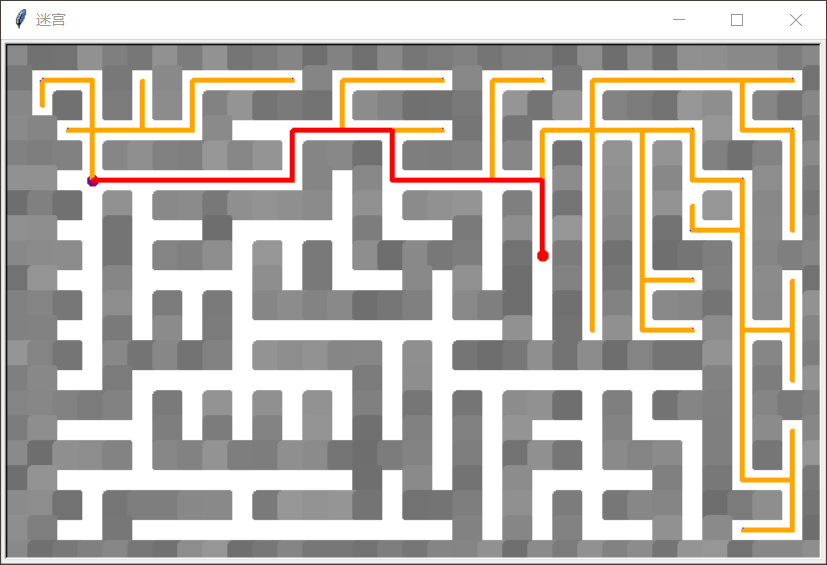
\includegraphics[scale=0.7]{img/C13/13-6/2.png}
	\end{figure}
\end{tcolorbox}